\documentclass[tikz, preview]{standalone}
%LOAD PACKAGES--------------------------------------------

\usepackage{amsfonts, amsthm, amssymb, amsmath, stmaryrd, etoolbox}
\usepackage{comment}
\usepackage{mathtools}
\usepackage{graphicx,caption,subcaption}
\usepackage{todonotes}
\usepackage{xcolor}

\usepackage[inline]{enumitem}
\setlist{itemsep=0em, topsep=0em, parsep=0em}
\setlist[enumerate]{label=(\alph*)}

\usepackage{tikz}
\usepackage[all,2cell]{xy}
\usetikzlibrary{matrix,arrows,shapes,decorations.markings,decorations.pathreplacing}
\definecolor{rewritecolor}{rgb}{0,.9,1}
\tikzset{rewritenode/.style={shape=circle,fill=rewritecolor,scale=0.25,font=\Huge}}
\tikzset{RWopen/.style={shape=circle,draw=black,fill=white,scale=0.5,font=\Huge}}
\tikzset{RWclosed/.style={shape=circle,fill=black,scale=0.5,font=\Huge}}
\tikzset{CDnode/.style={shape=circle,fill=white,scale=.5}}
\tikzset{zxgreen/.style={shape=circle,draw,thick,fill=green}}
\tikzset{zxred/.style={shape=circle,draw,thick,fill=red}}
\tikzset{zxyellow/.style={shape=rectangle,draw,thick,fill=yellow}}
\tikzset{zxdiamond/.style={shape=diamond,fill=black,inner sep=2.75}}
\tikzset{zxopen/.style={shape=circle,draw,thick,inner sep=2pt}}
\tikzset{->-/.style={decoration={%
			markings,
			mark=at position .5 with {\arrow{>}}},postaction={decorate}}
}
\tikzset{->-pos/.style={decoration={%
			markings,
			mark=at position #1 with {\arrow{>}}},postaction={decorate}}
}

\usepackage{hyperref}
\definecolor{hyperrefcolor}{rgb}{0,0,0.7}
\hypersetup{colorlinks,linkcolor={hyperrefcolor},citecolor={hyperrefcolor},urlcolor={hyperrefcolor}}

%NEW COMMANDS---------------------------------------------

\newcommand{\RR}{\mathbb{R}}
\newcommand{\ZZ}{\mathbb{Z}}
\newcommand{\NN}{\mathbb{N}}
\newcommand{\QQ}{\mathbb{Q}}
\newcommand{\CC}{\mathbb{C}}
\renewcommand{\epsilon}{\varepsilon}

\newcommand{\cl}[1]{\mathcal{#1}}
\newcommand{\scr}[1]{\mathscr{#1}}
\newcommand{\op}[1]{\operatorname{#1}}
\newcommand{\cat}[1]{\mathbf{#1}}
\newcommand{\dblcat}[1]{\mathbb{#1}}
\renewcommand{\t}[1]{\textup{#1}}

\newcommand{\from}{\colon}
\newcommand{\xto}[1]{\xrightarrow{#1}}
\newcommand{\sm}{\smallsetminus}
\newcommand{\tospan}{\xrightarrow{\mathit{sp}}}
\newcommand{\tocospan}{\xrightarrow{\mathit{csp}}}

%\newcommand{\diagram}[1]{\raisebox{-0.5\height}{\includegraphics{#1}}}

\newcommand{\bluebullet}{\textcolor{rewritecolor}{\bullet}}

%  macros for (co)span bicategories
\newcommand{\bispmap}[1]{\mathbf{Sp(#1)}}
\newcommand{\dblspmap}[1]{\mathbb{S}\mathbf{p(#1)}}
\newcommand{\bicspmap}[1]{\mathbf{Csp(#1)}}
\newcommand{\dblcspmap}[1]{\mathbb{C}\mathbf{sp(#1)}}
\newcommand{\bispsp}[1]{\mathbf{Sp(Sp(#1))}}
\newcommand{\dblspsp}[1]{\mathbb{S}\mathbf{p(Sp(#1))}}
\newcommand{\bicspcsp}[1]{\mathbf{Csp(Csp(#1))}}
\newcommand{\dblcspcsp}[1]{\mathbb{C}\mathbf{sp(Csp(#1))}}
\newcommand{\bimonspcsp}[1]{\mathbf{MonicSp(Csp(#1))}}
\newcommand{\dblmonspcsp}[1]{\mathbb{M}\mathbf{onicSp(Csp(#1))}}
\newcommand{\biepiccspsp}[1]{\mathbf{EpicCsp(Sp(#1))}}
\newcommand{\dblepiccspsp}[1]{\mathbb{E}\mathbf{picCsp(Sp(#1))}}

% defining arrow with a vertical line through it
\makeatletter
\def\slashedarrowfill@#1#2#3#4#5{%
	$\m@th\thickmuskip0mu\medmuskip\thickmuskip\thinmuskip\thickmuskip
	\relax#5#1\mkern-7mu%
	\cleaders\hbox{$#5\mkern-2mu#2\mkern-2mu$}\hfill
	\mathclap{#3}\mathclap{#2}%
	\cleaders\hbox{$#5\mkern-2mu#2\mkern-2mu$}\hfill
	\mkern-7mu#4$%
}
\def\rightslashedarrowfill@{%
	\slashedarrowfill@\relbar\relbar\mapstochar\rightarrow}
\newcommand{\xslashedrightarrow}[2][]{%
	\ext@arrow 0055{\rightslashedarrowfill@}{#1}{#2}}
\makeatother

\newcommand{\hto}{\xslashedrightarrow{}}


%DECLARE MATH OPERATORS----------------------------------

\DeclareMathOperator{\Hom}{Hom}
\DeclareMathOperator{\id}{id}
\DeclareMathOperator{\ob}{Ob}
\DeclareMathOperator{\arr}{arr}
\DeclareMathOperator{\im}{im}
\DeclareMathOperator{\Aut}{Aut}
\DeclareMathOperator{\Bij}{Bij}
\DeclareMathOperator{\Sub}{Sub}

%ENVIRONMENTS AND COUNTERS---------------------------------

\newtheorem{thm}{Theorem}[section]
\newtheorem{lem}[thm]{Lemma}
\newtheorem{prop}[thm]{Proposition}
\newtheorem{cor}[thm]{Corollary}

\theoremstyle{remark}
\newtheorem{remark}[thm]{Remark}
\newtheorem{notation}[thm]{Notation}

\theoremstyle{definition}
\newtheorem{ex}[thm]{Example} 
\newtheorem{defn}[thm]{Definition}

%\setcounter{tocdepth}{1} % Sets depth for table of contents. 

% FOR THIS PAPER ONLY

\newcommand{\zx}{_{\text{zx}}}
\newcommand{\bicat}[1]{\underline{\mathbf{#1}}}

\begin{document}
\[
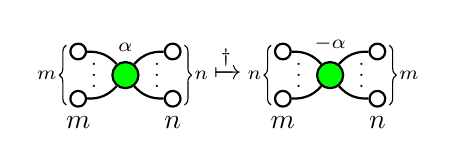
\begin{tikzpicture}
\begin{scope}[shift={(-1.3,0)}]
\node [zxgreen,label={[shift={(0,0)}]\scriptsize $\alpha$}] (v1) at (0,0) {};
\node [zxopen] (v2) at (-0.6,0.3) {};
\node [zxopen] (v3) at (-0.6,-0.3) {};
\node [zxopen] (v4) at (0.6,0.3) {};
\node [zxopen] (v5) at (0.6,-0.3) {};
\node at (-0.4,0.1) {\scriptsize $\vdots$};
\node at (0.4,0.1) {\scriptsize $\vdots$};
%
\draw  (v1) edge [thick,bend right=25] (v2);
\draw  (v1) edge [thick,bend left=25] (v3);
\draw  (v1) edge [thick,bend left=25] (v4);
\draw  (v1) edge [thick,bend right=25] (v5);
\draw[decoration={brace,mirror,raise=2pt},decorate]
(v2.north west) -- node[left=2pt] {\scriptsize $m$} (v3.south west); 
\draw[decoration={brace,raise=2pt},decorate]
(v4.north east) -- node[right=2pt] {\scriptsize $n$} (v5.south east); 
\node at (-0.6,-0.6) {$m$};
\node at (0.6,-0.6) {$n$};
\end{scope}
%
%
%
\node at (0,0.15) {$\xmapsto{\dagger}$};
%
%
%
\begin{scope}[shift={(1.3,0)}]
\node [zxgreen,label={[shift={(0,0)}]\scriptsize $-\alpha$}] (v1) at (0,0) {};
\node [zxopen] (v2) at (-0.6,0.3) {};
\node [zxopen] (v3) at (-0.6,-0.3) {};
\node [zxopen] (v4) at (0.6,0.3) {};
\node [zxopen] (v5) at (0.6,-0.3) {};
\node at (-0.4,0.1) {\scriptsize $\vdots$};
\node at (0.4,0.1) {\scriptsize $\vdots$};
%
\draw  (v1) edge [thick,bend right=25] (v2);
\draw  (v1) edge [thick,bend left=25] (v3);
\draw  (v1) edge [thick,bend left=25] (v4);
\draw  (v1) edge [thick,bend right=25] (v5);
\draw[decoration={brace,mirror,raise=2pt},decorate]
(v2.north west) -- node[left=2pt] {\scriptsize $n$} (v3.south west); 
\draw[decoration={brace,raise=2pt},decorate]
(v4.north east) -- node[right=2pt] {\scriptsize $m$} (v5.south east); 
\node at (-0.6,-0.6) {$m$};
\node at (0.6,-0.6) {$n$};
\end{scope}
\end{tikzpicture}
\]
\end{document}
